\documentclass[12pt,oneside]{book}
\usepackage{geometry}                		% See geometry.pdf to learn the layout options. There are lots.
\geometry{a4paper}                   			% ... or a4paper or a5paper or ... 
%\geometry{landscape}                		% Activate for for rotated page geometry
%\usepackage[parfill]{parskip}    		% Activate to begin paragraphs with an empty line rather than an indent
\usepackage{graphicx}				% Use pdf, png, jpg, or epsß with pdflatex; use eps in DVI mode
								% TeX will automatically convert eps --> pdf in pdflatex		
\usepackage{amssymb}

\usepackage[spanish]{babel}			% Permite que partes automáticas del documento aparezcan en castellano.
\usepackage[utf8]{inputenc}			% Permite escribir tildes y otros caracteres directamente en el .tex
\usepackage[T1]{fontenc}				% Asegura que el documento resultante use caracteres de una fuente apropiada.

\usepackage{hyperref}				% Permite poner urls y links dentro del documento

\title{Mi Juego Favorito}
\author{Javier Tibau}
%\date{}							% Activate to display a given date or no date

\begin{document}
\maketitle
\tableofcontents

\chapter{Introducción}
El libro a continuación es creado como una herramienta para el desarrollo de habilidades de edición colaborativa de documentos de texto plano. La herramienta que habilita dicha colaboración, en este taller, es Git pero podría ser reemplazada por otros sistemas de versionamiento.

\chapter{Los Juegos}

\section{Buscaminas}

\begin{figure}[htbp]
\begin{center}
\includegraphics[width=.60\textwidth]{./imagenes/minesweeper.png}
\caption{Buscaminas}
\label{Buscaminas}
\end{center}
\end{figure}
Buscaminas\footnote{\url{http://minesweeperonline.com/}} es uno de los juegos más jugados debido a lo ubicuo de su distribución. Fue incluido en 1992 en la versión de Windows 3.1 y desde entonces lo hemos encontrado presente en todas las versiones de dicho sistema operativo.
En la figura \ref{Buscaminas} puede ver una implementación web del juego.
La premisa del juego es simple: Limpiar el campo de juego sin hacer explotar ninguna de las minas que se encuentran en la cuadrícula.

\subsubsection{¿Por qué es uno de mis juegos favoritos?}
\begin{itemize}
\item[Javier Tibau] Las reglas del juego son sencillas y fáciles de entender. A pesar de esto, el juego no es atractivo para todo el mundo, creo que es un gusto adquirido. Las reglas me fueron presentadas por mi papá, quien en su máquina de trabajo con Windows 3.11 era uno de los pocos juegos ``divertidos'' que tenía. Para mi, el gran interés del juego es que destaca (o esconde) la resolución de problemas con fondo algebraico. En cierto momento del juego, y para el jugador que ha estudiado álgebra lineal, el reventar una casilla se torna similar a descifrar un sistema de ecuaciones con varias incógnitas. Los sistemas sencillos son bien definidos y tienen 2, 3 o hasta 4 incógnitas, mientras los más complejos pueden inclusive tener múltiples soluciones.
\end{itemize}

\section{Dota 2}

\begin{figure}[htbp]
\begin{center}
\includegraphics[width=.60\textwidth]{./imagenes/dota2.jpg}
\caption{Dota 2}
\label{Dota 2}
\end{center}
\end{figure}
Dota 2 \footnote{\url{http://dota2.com/}} es un juego creado por Valve basado en el popular mod de Warcraft 3, Defense of the Ancients. Es un juego de estrategia en equipo para ser jugado con equipos de 5 personas cada uno.
Dota 2 combina elementos de estrategia en tiempo real con perspectiva "en tercera persona", incorporando a todo ello un sistema de nivelación y jugabilidad de diversos juegos de rol como Diablo. Los jugadores asumen el papel de una unidad clasificado como un "héroe", que puede subir de nivel hasta un máximo de 25. La configuración básica de Dota 2 consiste en dos ciudades de distinta forma, cada una cuenta con una fortaleza de defensa conocida como "ancestro", situadas en los extremos opuestos de un mapa equilibrado de manera uniforme. Entre ellas hay varias regiones de conexión identificado como "caminos", que son atravesados por unidades enemigas, al tiempo que luchan contra poderosas torres defensivas a lo largo del camino. Los jugadores se dividen entre dos equipos, cada uno con hasta cinco jugadores, para competir como los principales defensores de cada Fortaleza de los Ancestros.

\subsubsection{¿Por qué es uno de mis juegos favoritos?}
\begin{itemize}
\item[Victor Cedeño] Este es un juego que requiere de comunicación y cooperación entre 5 personas para poder lograr el objetivo de vencer al otro equipo. Es muy dificil jugar solo sin la ayuda de tus compañeros. El juego tiene una gran selección de más de 100 heroes para elegir, esto quiere decir que cada partida es diferente ya que las combinaciones posibles de los equipos son innumerables. Es un juego que fomenta el trabajo en equipo y las decisiones correctas.
\end{itemize}

\include{juegos/Zelda}
\section{Deus Ex: Human Revolution}

\begin{figure}[htbp]
\begin{center}
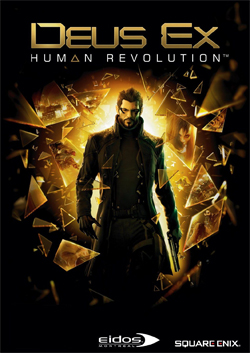
\includegraphics[width=.60\textwidth]{./imagenes/deusex.jpg}
\caption{Deus Ex: Human Revolution}
\label{Deus Ex: Human Revolution}
\end{center}
\end{figure}
Deus Ex: Human Revolution\footnote{\url{http://www.deusex.com/}}  es la precuela del aclamado "Deus Ex", lanzada en Agosto del 2011 por Eidos Montreal. Es un juego que se lleva a cabo en un futuro no muy distante, donde las aumentaciones (implantes físicos) son cosas del día a día, y que dan poder a quién las tenga.
En medio de todo esto se encuentra el protagonista, Adam Jensen, el cual se ve inmerso en un complot que abarca el destino de la humanidad.

\subsubsection{¿Por qué es uno de mis juegos favoritos?}
\begin{itemize}
\item[Luis Vasquez] Como un fanático de la serie, me fué natural comprar este juego en el día de lanzamiento, y no fui decepcionado. A parte de la gran trama que este juego ofrece , la cual no le pide favores a la del original, este logra modernizar todos los aspectos de jugabilidad
de  Deus Ex, asi como ofrecer al jugador varias opciones de juego, uno puede elegir entre sigilosamente infiltrarse en la base enemiga sin ser visto, o simplemente asesinar a sangre fría a cualquiera que se te cruze en tu camino.
\end{itemize}



\chapter{Conclusiones}
Cuales juegos fueron más populares y un breve razonamiento del porqué.

\end{document}  
